\section{Active Learning \label{sec:active}}

Information theoretic approaches to active learning are popular because
they do not require \DIFdelbegin \DIFdel{\emph{a priori} knowledge of the loss function or test domain}\DIFdelend \DIFaddbegin \DIFadd{prior knowledge of loss functions or test domains}\DIFaddend .
The central goal of information theoretic active learning is 
to \DIFdelbegin \DIFdel{reduce uncertainty about the parameters using the Shannon entropy i.e. seek a }\DIFdelend \DIFaddbegin \DIFadd{identify the }\DIFaddend new data point \DIFdelbegin \DIFdel{$\x$ }\DIFdelend that maximizes the \DIFdelbegin \DIFdel{decrease in expected posterior entropy: 
}\DIFdelend \DIFaddbegin \DIFadd{expected reduction in
posterior entropy. For the problem of preference learning,
as described in Section \ref{sec:prefKernel}, this implies
identifying the new item features $\mathbf{x}_i$ and $\mathbf{x}_j$ that maximize
}\DIFaddend \begin{align}   
\DIFdelbegin %DIFDELCMD < \label{eqn:ent_change}
%DIFDELCMD <         \argmax%%%
\DIFdel{_{\x} }%DIFDELCMD < \ent[p(\param | \data)] %%%
\DIFdelend \DIFaddbegin \ent[\mathcal{P}(g|\mathcal{D})] \DIFaddend - \E_{\DIFdelbegin \DIFdel{p}\DIFdelend \DIFaddbegin \DIFadd{\mathcal{P}}\DIFaddend (\DIFdelbegin %DIFDELCMD < \y%%%
\DIFdelend \DIFaddbegin \DIFadd{y}\DIFaddend |\DIFdelbegin %DIFDELCMD < \x%%%
\DIFdelend \DIFaddbegin \DIFadd{\mathbf{x}_i,\mathbf{x}_j,}\DIFaddend \data)} \left[ \DIFdelbegin %DIFDELCMD < \ent[p(\param| \y, \x,\data)] %%%
\DIFdelend \DIFaddbegin \ent[\mathcal{P}(g|y,\mathbf{x}_i,\mathbf{x}_j,\data)]\DIFaddend \right]\,,
\DIFaddbegin \label{eqn:ent_change}
\DIFaddend \end{align}
\DIFdelbegin \DIFdel{The preference kernel means that the following derivation apply equally to GPC and preference learning, for the latter $\x$ denotes an input pair. $\param$ denotes the parameters of the model and
$\ent[p(\param | \data)]=-\int p(\param|\data')\log p(\param|\data') d\param$ }\DIFdelend \DIFaddbegin \DIFadd{where $\mathcal{D}$ are the user preferences observed so far and
$\ent[p(x)]=-\int p(x)\log p(x)\,dx$ is }\DIFaddend the Shannon entropy. 
\DIFdelbegin \DIFdel{Although this frameworkwas presented several decades ago }\DIFdelend \DIFaddbegin \DIFadd{This framework, which was originally proposed by }\DIFaddend \citep{lindley1956}\DIFdelbegin \DIFdel{it is not straightforward to apply }%DIFDELCMD < \eqref{eqn:ent_change} %%%
\DIFdel{to complicated }\DIFdelend \DIFaddbegin \DIFadd{,
is difficult to apply directly to non-parametric }\DIFaddend models such
as \DIFdelbegin \DIFdel{nonparametric processes; parameter posteriors are often high or even infinite dimensional so computing their entropies is intractable, or even poorly
defined . 
To avoid gridding parameter space (exponentially hard with dimensionality), or sampling (from which it is notoriously hard to estimate entropies }%DIFDELCMD < \citep{panzeri2007}%%%
\DIFdel{)}\DIFdelend \DIFaddbegin \DIFadd{those based on GPs. 
In these models, entropies can be poorly
defined or their comptuation can be intractable.
In practice}\DIFaddend , current approaches make \DIFdelbegin \DIFdel{Gaussian or low dimensional approximations to }\DIFdelend \DIFaddbegin \DIFadd{some form of 
approximation for the computation of }\DIFaddend the posterior entropy \citep{mackay1992,lawrence2002}. 
\DIFdelbegin \DIFdel{A }\DIFdelend \DIFaddbegin \DIFadd{However, a }\DIFaddend second computational difficulty arises; if \DIFdelbegin \DIFdel{one can query one of $Q_{\x}$ possible input points , and observe one of $Q_{\y}$ responses (for binary preference learning, $Q_{\y}=2$), then $\mathcal{O}(Q_{\x}Q_{\y})$, potentially expensive, }\DIFdelend \DIFaddbegin \DIFadd{$n$ new data points are
available for selection, with $|\{-1,1\}|=2$ possible values for $y$.
Then $\mathcal{O}(2n)$ potentially expensive }\DIFaddend posterior updates are required to \DIFdelbegin \DIFdel{calculate Eqn.}%DIFDELCMD < \,\eqref{eqn:ent_change}%%%
\DIFdelend \DIFaddbegin \DIFadd{find the maximizer
of (\ref{eqn:ent_change})}\DIFaddend ; one for every \DIFdelbegin \DIFdel{possible input and corresponding label}\DIFdelend \DIFaddbegin \DIFadd{available feature vector and possible class value}\DIFaddend .
For the \DIFdelbegin \DIFdel{model presented in this work}\DIFdelend \DIFaddbegin \DIFadd{multi-class preference model}\DIFaddend , each update \DIFdelbegin \DIFdel{requires running the full EP algorithm .
}\DIFdelend \DIFaddbegin \DIFadd{would require to re-run the proposed
approximate inference algorithm (see Section \ref{sec:EPinference}).  This would be too expensive in practice.
}\DIFaddend 

\DIFdelbegin \DIFdel{An important insight arises if we note that the objective in Eqn.
}%DIFDELCMD < \,\eqref{eqn:ent_change} %%%
\DIFdelend \DIFaddbegin \DIFadd{A solution consists in noting that (\ref{eqn:ent_change}) }\DIFaddend is equivalent to the conditional mutual information between \DIFdelbegin \DIFdel{the unknown output and the parameters, $\info[\param,\y\vert\x,\data]$}\DIFdelend \DIFaddbegin \DIFadd{$y$ and $g$}\DIFaddend .
Using this \DIFdelbegin \DIFdel{insight it is simple to show that the objective can be rearranged }\DIFdelend \DIFaddbegin \DIFadd{we can rearrange this equation }\DIFaddend to compute entropies in $\y$ space:
\begin{align}
\DIFdelbegin %DIFDELCMD < \argmax%%%
\DIFdel{_{\x} }%DIFDELCMD < \ent[p(\y \vert \x, \data)] %%%
\DIFdelend \DIFaddbegin \ent[\mathcal{P}(y|\mathbf{x}_i,\mathbf{x}_j,\data)] \DIFaddend - \E_{\DIFdelbegin \DIFdel{p}\DIFdelend \DIFaddbegin \DIFadd{\mathcal{P}}\DIFaddend (\DIFdelbegin %DIFDELCMD < \param%%%
\DIFdelend \DIFaddbegin \DIFadd{g}\DIFaddend |\data)}
\left[\DIFdelbegin \DIFdel{p(}%DIFDELCMD < \ent[\y \vert \x,\param)] %%%
\DIFdelend \DIFaddbegin \ent\left[ \DIFadd{\mathcal{P}(y|\mathbf{x}_i,\mathbf{x}_j,g)}\right]\DIFaddend \right]\,. \label{eqn:rearrangement} 
\end{align}
\DIFdelbegin \DIFdel{Eqn.}%DIFDELCMD < \,\eqref{eqn:rearrangement} %%%
\DIFdel{overcomes the challenges we described for Eqn.}%DIFDELCMD < \,\eqref{eqn:ent_change}%%%
\DIFdelend \DIFaddbegin \DIFadd{This overcomes the previous challenges}\DIFaddend . Entropies are now \DIFdelbegin \DIFdel{calculated }\DIFdelend \DIFaddbegin \DIFadd{evaluated }\DIFaddend in
output space, which \DIFdelbegin \DIFdel{usually }\DIFdelend has low dimension. \DIFdelbegin \DIFdel{Also $\param$ }\DIFdelend \DIFaddbegin \DIFadd{Futhermore, $g$ }\DIFaddend is now conditioned \DIFdelbegin \DIFdel{only on }\DIFdelend \DIFaddbegin \DIFadd{to }\DIFaddend $\data$,
so only $\mathcal{O}(1)$ \DIFdelbegin \DIFdel{posterior updates are required i.e. we need only }\DIFdelend \DIFaddbegin \DIFadd{updates of the posterior distribution are required. In particular,
we only need }\DIFaddend to recompute the posterior once per data point selected, not for every possible data point under consideration.
\DIFdelbegin \DIFdel{Eqn.}%DIFDELCMD < \,\eqref{eqn:rearrangement} %%%
\DIFdelend \DIFaddbegin \DIFadd{Expression (\ref{eqn:rearrangement}) }\DIFaddend also provides us with an \DIFdelbegin \DIFdel{interesting }\DIFdelend intuition about the objective;
we seek the \DIFdelbegin \DIFdel{$\x$ for which }\DIFdelend \DIFaddbegin \DIFadd{$\mathbf{x}_i$ and $\mathbf{x}_j$ for which a) }\DIFaddend the model is marginally
\DIFdelbegin \DIFdel{most uncertain about $\y$ (high $\ent[p(\y \vert \x, \data)]$) , but for which individual settings of the parameters are confident (low $\E_{p(\param|\data)} \left[p( \ent[\y \vert \x,\param] \right)]$).
Figure \ref{fig:BALD} demonstrates the importance of including this second term. }\DIFdelend \DIFaddbegin \DIFadd{uncertain about $y$ (high $\ent[\mathcal{P}(\y | \mathbf{x}_i,\mathbf{x}_j, \data)]$) and
b) the model is confident about the value of $g$ at that location
(low $\E_{\mathcal{P}(g|\data)} \left[\ent [ \mathcal{P}(y |\mathbf{x}_i,\mathbf{x}_j,g] \right)]$).
}\DIFaddend This can be interpreted as seeking the \DIFdelbegin \DIFdel{$\x$ for which
the parameters }\DIFdelend \DIFaddbegin \DIFadd{$\mathbf{x}_i$ and $\mathbf{x}_j$ for which
$g$, }\DIFaddend under the posterior\DIFdelbegin \DIFdel{disagree }\DIFdelend \DIFaddbegin \DIFadd{, disagrees the most }\DIFaddend about the outcome\DIFdelbegin \DIFdel{the most, so }\DIFdelend \DIFaddbegin \DIFadd{.
Therefore, }\DIFaddend we refer to this objective as Bayesian Active Learning by Disagreement (BALD).
\DIFdelbegin \DIFdel{Next, }\DIFdelend \DIFaddbegin \DIFadd{In the following section }\DIFaddend we show how \DIFdelbegin \DIFdel{to apply Eqn.
}%DIFDELCMD < \,\eqref{eqn:rearrangement} %%%
\DIFdel{to GPC; the algorithm }\DIFdelend \DIFaddbegin \DIFadd{(\ref{eqn:rearrangement}) can be applied to the problem of binary classification with GPs.
Section \ref{sec:prefKernel} shows that this
problem is equivalent to the learning of pairwise user preferences.
The proposed method }\DIFaddend is independent of the particular \DIFdelbegin \DIFdel{method of inference, so we no longer need to build our entropy calculation around the particular posterior approximation as }\DIFdelend \DIFaddbegin \DIFadd{approach used for inference, something which does not hold for
the techniques described }\DIFaddend in \citep{mackay1992, krishnapuram2004, lawrence2002}. 

\DIFaddbegin \subsection{\DIFadd{BALD in Binary Classification with GPs}}

\DIFaddend \begin{figure}
\DIFdelbeginFL %DIFDELCMD < \centering
%DIFDELCMD < %%%
%DIF < \resizebox{3in}{!}{
%DIFDELCMD < % This file was created by matlab2tikz v0.1.3.
% Copyright (c) 2008--2011, Nico Schlömer <nico.schloemer@gmail.com>
% All rights reserved.
% 
% The latest updates can be retrieved from
%   http://www.mathworks.com/matlabcentral/fileexchange/22022-matlab2tikz
% where you can also make suggestions and rate matlab2tikz.
% 
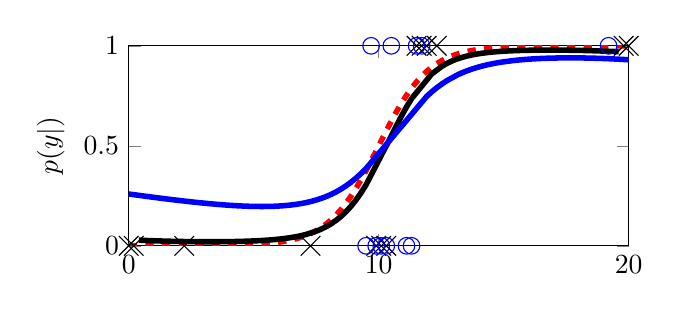
\begin{tikzpicture}

\begin{axis}[%
scale only axis,
width=2.5in,
height=1.0in,
xmin=0, xmax=20,
ymin=0, ymax=1,
ytick={0,0.5,1},
xtick = {0,10,20},
xlabel=$\x$,
ylabel=$p(y|\x)$,
legend style={ at={(1.0,0.05)}, anchor=south east}]
]
\addplot [
color=red,
line width=2.0pt,
dashed
]
coordinates{
 (0,4.53979e-005)(0.20202,5.55606e-005)(0.40404,6.79983e-005)(0.606061,8.322e-005)(0.808081,0.000101849)(1.0101,0.000124647)(1.21212,0.000152548)(1.41414,0.000186693)(1.61616,0.000228479)(1.81818,0.000279615)(2.0202,0.000342191)(2.22222,0.000418767)(2.42424,0.000512469)(2.62626,0.000627125)(2.82828,0.000767413)(3.0303,0.000939055)(3.23232,0.00114904)(3.43434,0.00140592)(3.63636,0.00172013)(3.83838,0.0021044)(4.0404,0.00257431)(4.24242,0.00314881)(4.44444,0.00385103)(4.64646,0.00470911)(4.84848,0.00575729)(5.05051,0.00703712)(5.25253,0.00859899)(5.45455,0.0105038)(5.65657,0.0128252)(5.85859,0.0156515)(6.06061,0.0190885)(6.26263,0.0232625)(6.46465,0.0283229)(6.66667,0.0344452)(6.86869,0.0418339)(7.07071,0.0507244)(7.27273,0.0613831)(7.47475,0.0741067)(7.67677,0.0892171)(7.87879,0.107052)(8.08081,0.127952)(8.28283,0.152236)(8.48485,0.180177)(8.68687,0.211963)(8.88889,0.247664)(9.09091,0.287186)(9.29293,0.330246)(9.49495,0.376355)(9.69697,0.424817)(9.89899,0.474769)(10.101,0.525231)(10.303,0.575183)(10.5051,0.623645)(10.7071,0.669754)(10.9091,0.712814)(11.1111,0.752336)(11.3131,0.788037)(11.5152,0.819823)(11.7172,0.847764)(11.9192,0.872048)(12.1212,0.892948)(12.3232,0.910783)(12.5253,0.925893)(12.7273,0.938617)(12.9293,0.949276)(13.1313,0.958166)(13.3333,0.965555)(13.5354,0.971677)(13.7374,0.976737)(13.9394,0.980911)(14.1414,0.984349)(14.3434,0.987175)(14.5455,0.989496)(14.7475,0.991401)(14.9495,0.992963)(15.1515,0.994243)(15.3535,0.995291)(15.5556,0.996149)(15.7576,0.996851)(15.9596,0.997426)(16.1616,0.997896)(16.3636,0.99828)(16.5657,0.998594)(16.7677,0.998851)(16.9697,0.999061)(17.1717,0.999233)(17.3737,0.999373)(17.5758,0.999488)(17.7778,0.999581)(17.9798,0.999658)(18.1818,0.99972)(18.3838,0.999772)(18.5859,0.999813)(18.7879,0.999847)(18.9899,0.999875)(19.1919,0.999898)(19.3939,0.999917)(19.596,0.999932)(19.798,0.999944)(20,0.999955) 
};
\label{GPplot:true}
%\addlegendentry{\scriptsize true gen. fun.}

\addplot [
color=black,
mark size=5.0pt,
only marks,
mark=x,
mark options={solid},
%forget plot
]
coordinates{
 (2.22222,0)(12.3232,1)(7.27273,0)(20,1)(9.89899,0)(11.9192,1)(0,0) 
};
%\addlegendentry{\scriptsize samples from BALD}

\addplot [
color=black,
mark size=5.0pt,
only marks,
mark=x,
mark options={solid},
%forget plot
]
coordinates{
 (10.303,0)(19.798,1) 
};
\label{GPplot:BALDsamp}

\addplot [
color=black,
mark size=5.0pt,
only marks,
mark=x,
mark options={solid},
%forget plot
]
coordinates{
 (11.5152,1)(10.101,0) 
};

\addplot [
color=black,
mark size=5.0pt,
only marks,
mark=x,
mark options={solid}
]
coordinates{
 (0.20202,0)(11.7172,1) 
};

\addplot [
color=blue,
mark size=3.0pt,
only marks,
mark=o,
mark options={solid},
%forget plot
]
coordinates{
 (11.1111,0)(19.1919,1) 
};
\label{GPplot:MESsamp}
%\addlegendentry{\scriptsize samples from MES}

\addplot [
color=blue,
mark size=3.0pt,
only marks,
mark=o,
mark options={solid},
%forget plot
]
coordinates{
 (11.5152,1)(10.303,0) 
};

\addplot [
color=blue,
mark size=3.0pt,
only marks,
mark=o,
mark options={solid},
%forget plot
]
coordinates{
 (11.3131,0)(11.7172,1) 
};

\addplot [
color=blue,
mark size=3.0pt,
only marks,
mark=o,
mark options={solid},
%forget plot
]
coordinates{
 (10.5051,1)(9.89899,0) 
};

\addplot [
color=blue,
mark size=3.0pt,
only marks,
mark=o,
mark options={solid}
]
coordinates{
 (10.101,0)(9.69697,1)(9.49495,0) 
};

\addplot [
color=black,
solid,
line width=2.0pt
]
coordinates{
 (0.40404,0.0283168)(0.606061,0.0272039)(0.808081,0.0261815)(1.0101,0.0252468)(1.21212,0.0243974)(1.41414,0.0236309)(1.61616,0.0229454)(1.81818,0.0223395)(2.0202,0.0218118)(2.42424,0.0209891)(2.62626,0.0206944)(2.82828,0.0204787)(3.0303,0.0203439)(3.23232,0.0202927)(3.43434,0.020329)(3.63636,0.0204578)(3.83838,0.0206856)(4.0404,0.0210203)(4.24242,0.0214721)(4.44444,0.0220533)(4.64646,0.0227792)(4.84848,0.0236682)(5.05051,0.0247431)(5.25253,0.0260315)(5.45455,0.027567)(5.65657,0.0293907)(5.85859,0.0315525)(6.06061,0.0341134)(6.26263,0.0371474)(6.46465,0.0407449)(6.66667,0.0450154)(6.86869,0.0500919)(7.07071,0.0561342)(7.47475,0.071919)(7.67677,0.0821554)(7.87879,0.0943502)(8.08081,0.108849)(8.28283,0.126031)(8.48485,0.146291)(8.68687,0.170023)(8.88889,0.197579)(9.09091,0.229232)(9.29293,0.265119)(9.49495,0.305188)(10.5051,0.549174)(10.7071,0.599838)(10.9091,0.648411)(11.1111,0.693916)(11.3131,0.735619)(12.1212,0.859273)(12.5253,0.897445)(12.7273,0.911956)(12.9293,0.923989)(13.1313,0.933938)(13.3333,0.942151)(13.5354,0.948926)(13.7374,0.954516)(13.9394,0.959133)(14.1414,0.962948)(14.3434,0.966104)(14.5455,0.968714)(14.7475,0.970871)(14.9495,0.972651)(15.1515,0.974114)(15.3535,0.975308)(15.5556,0.976272)(15.7576,0.977039)(15.9596,0.977635)(16.1616,0.978079)(16.3636,0.978389)(16.5657,0.978577)(16.7677,0.978655)(16.9697,0.978632)(17.1717,0.978513)(17.3737,0.978304)(17.5758,0.978009)(17.7778,0.977632)(17.9798,0.977173)(18.1818,0.976635)(18.3838,0.976017)(18.5859,0.97532)(18.7879,0.974543)(18.9899,0.973686)(19.1919,0.972748)(19.3939,0.971726)(19.596,0.970619) 
};
\label{GPplot:BALD}
%\addlegendentry{\scriptsize post. mean (BALD)}

\addplot [
color=blue,
solid,
line width=2.0pt
]
coordinates{
 (0,0.259156)(0.20202,0.255723)(0.40404,0.25232)(0.606061,0.248951)(0.808081,0.24562)(1.0101,0.242332)(1.21212,0.239092)(1.41414,0.235905)(1.61616,0.232776)(1.81818,0.229712)(2.0202,0.226718)(2.22222,0.223803)(2.42424,0.220972)(2.62626,0.218235)(2.82828,0.2156)(3.0303,0.213077)(3.23232,0.210676)(3.43434,0.208409)(3.63636,0.206287)(3.83838,0.204326)(4.0404,0.20254)(4.24242,0.200946)(4.44444,0.199564)(4.64646,0.198414)(4.84848,0.197521)(5.05051,0.19691)(5.25253,0.196613)(5.45455,0.196662)(5.65657,0.197098)(5.85859,0.197963)(6.06061,0.199307)(6.26263,0.201188)(6.46465,0.203668)(6.66667,0.206823)(6.86869,0.210734)(7.07071,0.215497)(7.27273,0.221216)(7.47475,0.228012)(7.67677,0.236013)(7.87879,0.245364)(8.08081,0.256215)(8.28283,0.268728)(8.48485,0.283059)(8.68687,0.299362)(8.88889,0.317769)(9.09091,0.338377)(9.29293,0.361234)(9.49495,0.386321)(11.9192,0.747094)(12.1212,0.769891)(12.3232,0.790536)(12.5253,0.809094)(12.7273,0.825675)(13.1313,0.853482)(13.3333,0.865021)(13.5354,0.875194)(13.7374,0.884149)(13.9394,0.892023)(14.1414,0.898941)(14.3434,0.905015)(14.5455,0.910342)(14.7475,0.915009)(14.9495,0.919093)(15.3535,0.925764)(15.5556,0.928457)(15.7576,0.930781)(15.9596,0.932772)(16.1616,0.934462)(16.3636,0.935877)(16.5657,0.937041)(16.7677,0.937974)(16.9697,0.938693)(17.1717,0.939212)(17.3737,0.939545)(17.5758,0.939701)(17.7778,0.939689)(17.9798,0.939519)(18.1818,0.939195)(18.3838,0.938725)(18.5859,0.938111)(18.7879,0.937359)(18.9899,0.936472)(19.3939,0.934303)(19.596,0.933025)(19.798,0.931621)(20,0.930093) 
};
\label{GPplot:MES}
%\addlegendentry{\scriptsize post. mean (MES)}


\end{axis}
\end{tikzpicture}
%%%
\DIFdelendFL \DIFaddbeginFL 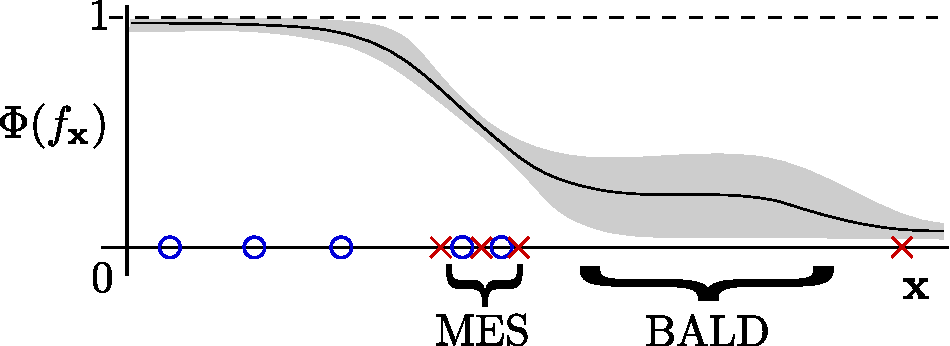
\includegraphics[scale = 0.5]{figs/BALD_eg.pdf} \DIFaddendFL \\
%DIF < }
\vskip\DIFdelbeginFL \DIFdelFL{-0.5cm
}\DIFdelendFL \DIFaddbeginFL \DIFaddFL{-0.4cm
}\DIFaddendFL \caption{\DIFdelbeginFL \DIFdelFL{1D toy }\DIFdelendFL \DIFaddbeginFL \DIFaddFL{Toy }\DIFaddendFL GPC example \DIFaddbeginFL \DIFaddFL{with 1D input}\DIFaddendFL . \DIFdelbeginFL \DIFdelFL{True data generating function (\ref{GPplot:true}) is random at $\x=10$. (\ref{GPplot:BALDsamp}), (\ref{GPplot:MESsamp}) }\DIFdelendFL \DIFaddbeginFL \DIFaddFL{Cirles and crosses }\DIFaddendFL denote \DIFaddbeginFL \DIFaddFL{previosuly seen }\DIFaddendFL samples\DIFdelbeginFL \DIFdelFL{taken using }\DIFdelendFL \DIFaddbeginFL \DIFaddFL{. Plot shows the mean and variance of the GP predictive distribution trained upon these points. }\DIFaddendFL Maximum Entropy Sampling (MES, see Section \ref{sec:relatedWork}) \DIFdelbeginFL \DIFdelFL{and BALD respectively, (\ref{GPplot:BALD}) and (\ref{GPplot:MES}) are the GP posterior mean predictions after training on }\DIFdelendFL \DIFaddbeginFL \DIFaddFL{seeks its next datapoint in }\DIFaddendFL the \DIFdelbeginFL \DIFdelFL{samples selected by BALD and MES. MES uses only }\DIFdelendFL \DIFaddbeginFL \DIFaddFL{region of highest marginal uncertainty because it ignores }\DIFaddendFL the \DIFdelbeginFL \DIFdelFL{first }\DIFdelendFL \DIFaddbeginFL \DIFaddFL{second }\DIFaddendFL term in \DIFaddbeginFL \DIFaddFL{Eq.}\,\DIFaddendFL \eqref{eqn:rearrangement}, \DIFdelbeginFL \DIFdelFL{and samples excessively about $\x=10$ because uncertainty in the model parameters }\DIFdelendFL \DIFaddbeginFL \DIFaddFL{so nothing new }\DIFaddendFL is \DIFdelbeginFL \DIFdelFL{confounded with uncertainty in }\DIFdelendFL \DIFaddbeginFL \DIFaddFL{learned about }\DIFaddendFL the \DIFdelbeginFL \DIFdelFL{output}\DIFdelendFL \DIFaddbeginFL \DIFaddFL{data}\DIFaddendFL . BALD \DIFdelbeginFL \DIFdelFL{penalises $\x$'s for which the individual settings of }\DIFdelendFL \DIFaddbeginFL \DIFaddFL{will select }\DIFaddendFL the \DIFdelbeginFL \DIFdelFL{parameters do not predict }\DIFdelendFL \DIFaddbeginFL \DIFaddFL{next datapoint from }\DIFaddendFL the \DIFdelbeginFL \DIFdelFL{output with confidence}\DIFdelendFL \DIFaddbeginFL \DIFaddFL{region of greatest model uncertainty}\DIFaddendFL , \DIFdelbeginFL \DIFdelFL{hence selects more varied samples and yields a better posterior mean}\DIFdelendFL \DIFaddbeginFL \DIFaddFL{as indicated in the Figure}\DIFaddendFL . \label{fig:BALD}}
\end{figure}

\DIFdelbegin \subsection{\DIFdel{Application to GP Preference Learning}}
%DIFAUXCMD
\addtocounter{subsection}{-1}%DIFAUXCMD
\DIFdel{Here we apply Eqn.}%DIFDELCMD < \,\eqref{eqn:rearrangement} %%%
\DIFdel{to GPC where the latent function $\latfun$ is the model parameters ($\param$ in the previous section). As for our hybrid EP algorithm, all the standard approximate inference algorithms for GPC model the posterior with
a Gaussian e.g. Laplace approximation , sparse methods; the
following derivations apply equally to these scenarios. The symbol }%DIFDELCMD < {\scriptsize%%%
\DIFdel{$\stackrel{1}{\approx}$}%DIFDELCMD < } %%%
\DIFdel{denotes when such an approximation is exploited. The entropy of }\DIFdelend \DIFaddbegin \DIFadd{Most approximate inference methods for }\DIFaddend the \DIFdelbegin \DIFdel{binary output variable $\y$ given the latent function $\latfun$ }\DIFdelend \DIFaddbegin \DIFadd{problem of binary classification with
GPs produce a Gaussian approximation to the posterior distribution of $f$, the
latent function of interest. In the binary GPs classifier, the entropy of $y$ given the corresponding value of $f$ 
}\DIFaddend can be expressed in terms of the binary entropy function, \DIFdelbegin \DIFdel{$\mathrm{h}(q)=- q\log q - (1-q)\log(1-q)$:
}\DIFdelend \DIFaddbegin \DIFadd{$\mathrm{h}[f]=- f\log f - (1-f)\log(1-f)$.
In particular,
}\DIFaddend \begin{align}
\ent[p(y\vert\x,\latfun)] &= \mathrm{h}\DIFdelbegin %DIFDELCMD < \left(%%%
\DIFdelend \DIFaddbegin \left[\DIFaddend \Phi(\latfun(\x)\DIFdelbegin %DIFDELCMD < \right)%%%
\DIFdelend \DIFaddbegin \right]\DIFaddend \,. \notag
\end{align}
\DIFdelbegin \DIFdel{Expectations over the posterior need to be computed. Using the Gaussian approximationto the posterior, }\DIFdelend \DIFaddbegin \DIFadd{When the posterior distribution of $f$ is modeled using a Gaussian approximation, we have that
}\DIFaddend for each $\x$, $\latfun_{\x} = \latfun(\x)$ will follow a Gaussian distribution with mean $\mu_{\x}$ and
variance $\sigma_{\x}^2$.
The first term in \DIFdelbegin \DIFdel{Eqn.}%DIFDELCMD < \,\eqref{eqn:rearrangement}%%%
\DIFdelend \DIFaddbegin \DIFadd{(\ref{eqn:rearrangement}), that is}\DIFaddend , $\ent[p(y\vert\x,\data)]$\DIFaddbegin \DIFadd{, }\DIFaddend can be handled analytically \DIFaddbegin \DIFadd{in this case}\DIFaddend :
\begin{align}
\ent[p(y\vert\x,\data)] &\stackrel{1}{\approx} \mathrm{h}\DIFdelbegin %DIFDELCMD < \left( %%%
\DIFdelend \DIFaddbegin \left[ \DIFaddend \int \Phi( \latfun_{\x} )
\mathcal{N}(\latfun_{\x}| \mu_{\x},\sigma_{\x}^2) d\latfun_{\x} \DIFdelbegin %DIFDELCMD < \right) %%%
\DIFdelend \DIFaddbegin \right] \DIFaddend \notag \\ 
&= \mathrm{h} \DIFdelbegin %DIFDELCMD < \left( %%%
\DIFdelend \DIFaddbegin \left[ \DIFaddend \Phi\left( \frac{\mu_{\x}}{\sqrt{\sigma^2_{\x} + 1}} \right)\DIFdelbegin %DIFDELCMD < \right)%%%
\DIFdelend \DIFaddbegin \right]\DIFaddend \,\DIFdelbegin \DIFdel{. }\DIFdelend \DIFaddbegin \DIFadd{, }\DIFaddend \label{ent_mean}
\end{align}
\DIFaddbegin \DIFadd{where $\stackrel{1}{\approx}$ denotes the Gaussian approximation to the posterior of $\latfun_{\x}$.
}\DIFaddend The second term \DIFaddbegin \DIFadd{in (\ref{eqn:rearrangement}), that is}\DIFaddend ,
$\E_{p(\latfun\vert\data)} \left[ \ent[p(\y\vert\x, \latfun)] \right]$\DIFaddbegin \DIFadd{, }\DIFaddend can be computed approximately as follows:
\DIFdelbegin %DIFDELCMD < \vskip%%%
\DIFdel{-0.4cm
}%DIFDELCMD < {\small
%DIFDELCMD < %%%
\DIFdelend \begin{align}
\E_{p(f\vert\data)} \DIFaddbegin & \DIFaddend \left[ \ent[p(\y\vert\x, \latfun)] \right] \DIFdelbegin %DIFDELCMD < &%%%
\DIFdelend \stackrel{1}{\approx} \DIFdelbegin \DIFdel{\int \mathrm{h}(\Phi(}%DIFDELCMD < \latfun%%%
\DIFdel{_{\x})) }\DIFdelend \DIFaddbegin \notag \\
& \DIFadd{\int \mathrm{h}[\Phi(\latfun_{\x})] }\DIFaddend \mathcal{N}(\latfun_{\x}| \mu_{\x},\sigma_{\x}^2) d\latfun_{\x} \DIFdelbegin %DIFDELCMD < \label{eqn:mean_entropy}%%%
\DIFdelend \DIFaddbegin \stackrel{2}{\approx} \notag\DIFaddend \\
& \DIFdelbegin %DIFDELCMD < \stackrel{2}{\approx} %%%
\DIFdelend \int \exp\left(-\DIFdelbegin \DIFdel{\frac{\latfun_{\x}^2}{\pi\ln2}}\DIFdelend \DIFaddbegin \DIFadd{\frac{\latfun_{\x}^2}{\pi\log 2}}\DIFaddend \right) \mathcal{N}(\latfun_{\x}| \mu_{\x},\sigma_{\x}^2)d\latfun_{\x} \DIFaddbegin \DIFadd{= }\DIFaddend \notag\\ 
& \DIFdelbegin \DIFdel{= }\DIFdelend \frac{C}{\sqrt{\sigma_{\x}^2 + C^2}}\exp\left(-\frac{\mu_{\x}^2}{2\left(\sigma_{\x}^2 + C^2\right)}\right)\,,\notag
\end{align}
\DIFdelbegin %DIFDELCMD < }
%DIFDELCMD < %%%
\DIFdel{where $C=\sqrt{\frac{\pi\ln2}{2}}$. The integral in the left hand side of Eqn.}%DIFDELCMD < \,\eqref{eqn:mean_entropy} %%%
\DIFdel{is intractable. By performing a Taylor expansion on $\ln \mathrm{h}(\Phi(\latfun_{\x}))$ we can see that it can be approximated up to $\mathcal{O}(\latfun_{\x}^4)$ by a }\DIFdelend \DIFaddbegin \DIFadd{where $C=\sqrt{\pi\log 2 / 2}$ and $\stackrel{2}{\approx}$ denotes
an approximation to $\log \mathrm{h}[\Phi(\latfun_{\x})]$ given
by the }\DIFaddend squared exponential curve \DIFdelbegin \DIFdel{, $\exp(-\latfun_{\x}^2/\pi\ln2)$. 
We denote this approximation as }%DIFDELCMD < {\scriptsize %%%
\DIFdel{$\stackrel{2}{\approx}$}%DIFDELCMD < } %%%
\DIFdel{and note that it strikingly }\DIFdelend \DIFaddbegin \DIFadd{$\exp(-\latfun_{\x}^2/\pi\log 2)$. 
This approximation is very }\DIFaddend accurate (Taylor expansion and \DIFdelbegin \DIFdel{a }\DIFdelend vizualisation are presented in the supplementary material).
The maximum possible error incurred in the \DIFdelbegin \DIFdel{integral in Eqn.}%DIFDELCMD < \,\eqref{eqn:mean_entropy} %%%
\DIFdelend \DIFaddbegin \DIFadd{required integral }\DIFaddend is only $0.27\%$\DIFaddbegin \DIFadd{, }\DIFaddend which occurs when
$\mathcal{N}(\latfun_{\x}| \mu_{\x},\sigma_{\x}^2)$ is centred at $\mu_{\x}=\pm 2.05$  with $\sigma_{\x}^2$ \DIFdelbegin \DIFdel{tends }\DIFdelend \DIFaddbegin \DIFadd{tending }\DIFaddend to zero.
\DIFdelbegin \DIFdel{We can now apply the standard convolution formula for Gaussians to get a closed form expression for both terms of Eqn.}%DIFDELCMD < \,\eqref{eqn:rearrangement}%%%
\DIFdel{.
}\DIFdelend 

To summarize, the BALD algorithm for \DIFdelbegin \DIFdel{GPC}\DIFdelend \DIFaddbegin \DIFadd{active binary GP classification }\DIFaddend / preference learning first applies
any approximate inference \DIFdelbegin \DIFdel{algorithm (for us, EP) }\DIFdelend \DIFaddbegin \DIFadd{method }\DIFaddend to obtain the posterior \DIFdelbegin \DIFdel{predictive }\DIFdelend mean
$\mu_{\x}$ and variance $\sigma_{\x}^2$ \DIFdelbegin \DIFdel{for }\DIFdelend \DIFaddbegin \DIFadd{of $f$ at }\DIFaddend each point of interest $\x$. Then, it selects the
\DIFdelbegin \DIFdel{preference data point/pair }\DIFdelend \DIFaddbegin \DIFadd{data }\DIFaddend $\x$ that maximizes the \DIFdelbegin \DIFdel{following objective
function:
}%DIFDELCMD < \begin{equation}
\begin{displaymath}%DIFAUXCMD
%DIFDELCMD <         %%%
\DIFdel{\mathrm{h} }%DIFDELCMD < \left( %%%
\end{displaymath}%DIFAUXCMD
\DIFdelend \DIFaddbegin \DIFadd{objective
}\begin{align}
& \DIFadd{\mathrm{h} }\left[ \DIFaddend \Phi\left(  \frac{\mu_{\x}}{\sqrt{\sigma^2_{\x} + 1}} \right)\DIFdelbegin %DIFDELCMD < \right) %%%
\DIFdelend \DIFaddbegin \right] \DIFaddend -\DIFaddbegin \notag \\
& \DIFadd{\hspace{2cm} }\DIFaddend \frac{C}{\sqrt{\sigma_{\x}^2 + C^2}} \exp\left(-\frac{\mu_{\x}^2}{2\left(\sigma_{\x}^2 + C^2\right)}\right)\,.\label{eqn:BALD}
\DIFdelbegin %DIFDELCMD < \end{equation}
\end{align}%DIFAUXCMD
%DIFDELCMD < %%%
%DIF < For most practically relevant kernels, the objective \eqref{eqn:BALD} is a smooth and differentiable function of $\x$, so should we be able to select items from a continuous feature space gradient-based optimisation methods can be employed.
%DIFDELCMD < 

%DIFDELCMD < %%%
%DIF < In this section we describe the general framework for our information-theoretic approach to active learning and describe the computational advantages. We then derive how to compute the information theoretic objective with very minimal approximations for our preference learning model. Note that due to the kernel reformulation in \ref{sec:prefKernel}, the equations in this section are exactly the same as for deriving the equivalent active learning algorithm for GP classification. For this reason, and to keep notation clean, we refer to an input datapoint as $\x$, although for our preference learning model this refers to a pair of input items. 
%DIFDELCMD < 

%DIFDELCMD < %%%
%DIF < Data points $\data'$ are selected that satisfy $\argmin_{\data'}\ent[p(\param|\data')]=-\int p(\param|\data')\log p(\param|\data') d\param$, where $\param$ to denotes the parameters of the model; for multi-task preference learning, these parameters correspond to the latent functions $g$ for each user. Solving this problem is NP-hard, however, as is common in sequential decision making tasks a myopic (greedy) approximation is made \citep{heckerman1995}. It has been shown that the myopic policy can perform near-optimally \citep{dasgupta2005,golovin2010}. Therefore, the objective is to seek a new preference data point $\x$ that maximises the decrease in expected posterior entropy:
%DIFDELCMD < 

%DIFDELCMD <  %%%
\begin{align}%DIFAUXCMD
\DIFdelend \DIFaddbegin \end{align}
 \DIFaddend